\chapter{Introduction}

\lepix{} is a small, general-purpose programming language whose goal is to make working with parallel computation and multidimensional arrays simple. Featuring a preprocessor, namespacing, sliced multidimensional array syntax, parallel blocks based on an invocation count and ID, and bottom-up type derivation (automatic type deduction), the goal of the language is to produce an environment that is heavily statically checked and ensures a degree of correctness the user of the language can rely on.

However, this implementation of \lepix{} specifically departed from some of the original design goals due to time constraints and team issues. Therefore, while parallelism and arrays were on the table, neither made it into the implementation in the given time frame I had to put the rest of the language (entire semantic analyzer plus all of the codegen) (about 2 weeks, plus post-mortem time). The implementation here instead set out to demonstrate how 4 techniques can be achieved with the language:

\begin{enumerate}
	\item Namespaces - namespacing as defined in the original language, but lacking using statements inside definition blocks
	\item Overloading - having multiple functions assigned to the same name, separated internally by a name-mangling scheme based on arity and arguments.
	\item Bottom-up Type Derivation - deduction of return types for functions based on the expression of returns (or none therein).
	\item Call targets as expressions - DICE\footnote{http://www.cs.columbia.edu/~sedwards/classes/2015/4115-fall/reports/Dice.pdf} and other languages -- including our own, at first -- implemented function calls as an identifier plus necessary function all syntax. This implementation of \lepix{} treats it as an expression, which presents unique challenges for the previous 2 goals. 
\end{enumerate}

\section{Language Proposal}

Below is our initial language proposal, in its entirety. It was very ambitious, and Professor Edwards told us to scale our goals back considerably. From it, we threw out GPU code generation in exchange for Parallelism and code generation for LLVM IR alone, and also wanted to focus on syntax for multidimensional arrays.

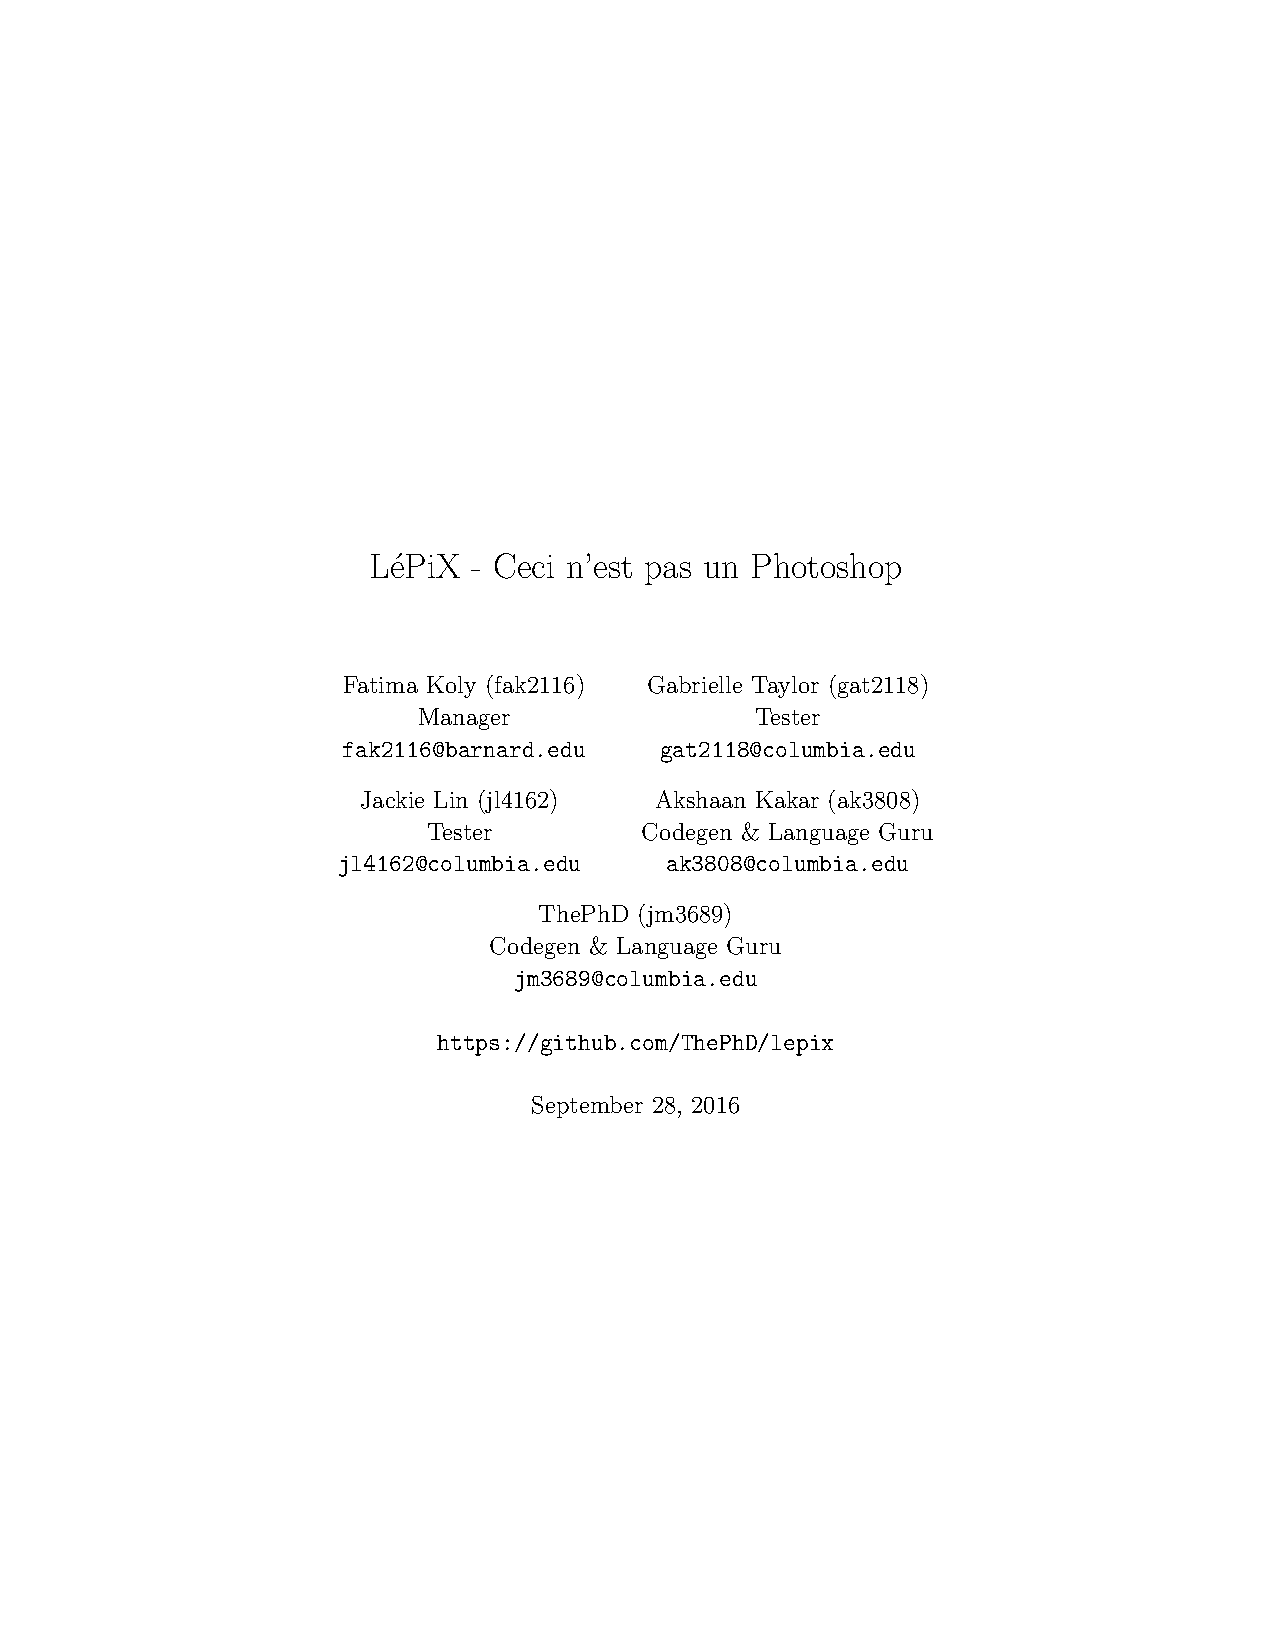
\includepdf[pages=-]{\detokenize{lp/lepix.pdf}}
